\documentclass[letterpaper,12pt]{article}
\usepackage[utf8]{inputenc}
\usepackage[english]{babel}
% \usepackage{setspace} % double spacing
% \doublespacing
\usepackage[nottoc]{tocbibind} %Adds "References" to the table of contents
\usepackage[colorlinks=true,linktocpage=true, allcolors=blue]{hyperref}
\usepackage[usenames, dvipsnames]{color}
\usepackage{csquotes} %Display quotes
\usepackage[linesnumbered,ruled]{algorithm2e} %Pesudocode
\DontPrintSemicolon
\SetKwInOut{Input}{Input}
\SetKwInOut{Output}{Output}
\SetKwRepeat{Do}{do}{while}

\usepackage{chngcntr}%ref for algorithm
\counterwithout{algocf}{section}
\counterwithout{algocf}{subsection}
\renewcommand{\thealgocf}{\arabic{section}.\arabic{subsection}.\arabic{algocf}}

\usepackage{amsthm} %write definition
\theoremstyle{definition}
\newtheorem{definition}{Definition}[section]
 
\usepackage{array}% for table

\usepackage{ amssymb } %math symbol

\usepackage{tikz}
\usetikzlibrary{positioning}
\usetikzlibrary{decorations.markings}
\usetikzlibrary{arrows.meta}

%Document title, author and date (empty)
\title{Course Scheduling Algorithm}
\author{Adviser: David Eppstein\
\and Student: Zhaohua Zeng}
\date{\today}

%Beginning of the document
\begin{document}

% introduction:
%% project problem
%% Why problem? significant problem
%% Lack insight on ... my insight
%% briefly introduce solution

% Related works
%% algorithms
%% cant solve this problem because....


% Proposed Method
%% problem formulation and term definition
%% step by step introduce my method
%% Time and space complexity
%%% lemma???

% Experimental Result

% Conclusion and future work






\maketitle

\tableofcontents
\newpage
\begin{abstract}
	By modifying the Coffman-Graham algorithm and the Hu’s algorithm, we give a scheduling algorithm that can output a course study plan for college students in $O(|V|^2)$ time. 
\end{abstract}
\section{Introduction}
% - Project Idea (put it in other places?)
% - Data structures (somewhere else)
%   - Course (vertex)
%   - Graph
% - Coffman-Graham Algorithm
% - Hu's Algorithm
% \subsection{Course Scheduling Problem} %Course scheduling problem
Consider the problem of scheduling courses for next quarter. To graduate on time, what courses should a Computer Science student choose in the next few quarters? Currently, many students, especially freshmen and transfer students, would like to ask school academic counselors for advice before enrolling to courses of next quarter. Since the number of counselors is limited but many students would go to the office for help, getting suggestions becomes time consuming. 

Although we find task scheduling algorithms giving a possible solution for the course scheduling problem, these algorithms do not consider some constraints that exist in this problem. Thus, we make modifications based on constraints after we adapt the labeling and scheduling phases in two task scheduling algorithms, the Coffman-Graham algorithm and Hu's algorithm. Our course scheduling algorithm can generate a reasonable schedule plan as a guidance for students. Using this algorithm, one can develop a tool that can help academic counselors shorten the time spent on arranging student schedules and provide accurate information. At the same time, students can check what series of courses they are required to take to satisfy some prerequisites and organize their study plans at ease.

Our course scheduling algorithm can:
\begin{enumerate}
\item Make a course schedule for the entire undergraduate/graduate path, which can satisfy school/major requirements;
\item Allow users to specify the maximum course units for a single quarter;
\item Allow users to start scheduling process from the half-way. With the information about what courses users have taken, and the starting quarter of the schedule, the algorithm can generate a study plan for the next few quarters until all specified requirements are satisfied; 
\item Allow users to avoid taking some courses.
\end{enumerate}
% We use Python to test the performance of the algorithm, and related code is hosted on a GitHub Repository~\footnote{\url{https://github.com/jennyzeng/CourseScheduling}}. 
\section{Related Works}
The Coffman-Graham algorithm and Hu's algorithm are related to precedence-constrained mulitprocessor scheduling problem, which is about minimizing the total makespan of the schedule. 
Let $V$ be a set of tasks with indices $1,2,\dot, n$, $G=(V,E)$ be an acyclic directed graph with $|V|$ tasks and $|E|$ edges. 
An edge $e=(u,v)$ for $u,v\in V$ is in $E$ if $u$ must be executed before $v$ is assigned to a processor. $W$ is the number of processors in the problem. Each task $v \in V$ takes 1 units of time to finish, each processor $w_j$ can only execute one task at a time. 
The problem is about scheduling $|V|$ tasks to $W$ multiprocessors. A layer $L_k$ with width $W$ is the assignments in time $t_k$ in the schedule $L$. 

Minimizing the total makespan of a schedule is equivalent to minimizing the number of layers. However, this problem is NP-complete, so both the Coffman-Graham algorithm and Hu's algorithm suggest heuristic methods for scheduling~\cite{battista_chapter_1998}.

There are some similarities between the precedence-constrained mulitprocessor scheduling problem and the course scheduling problem. First, we can view each task as a course in our problem, and each course also takes one unit of time to finish within one quarter. Then we can use a quarter as a time unit. Similar to the precedence-constrained relationship represented by edges between tasks, some courses have other courses as their prerequisites. It means students cannot take a course until they satisfy its prerequisites, so the course could only be assigned to a layer later than its prerequisites' layers. Moreover, although there is no exact number of processors in course scheduling problem, we can use maximum units per quarter as the width of a layer instead. Since we want to minimize the total number of quarters in the schedule, the goal of the course scheduling problem is also minimizing makespan. Consequently, we can transform the precedence-constrained mulitprocessor scheduling problem to the course scheduling problem and develop a new algorithm based on algorithms described below to solve the problem. 

\subsection{Coffman-Graham Algorithm}
The Coffman-Graham algorithm takes a reduced directed acyclic graph (DAG) $G=(V,E)$ and a positive integer $W$, width of the layer, as inputs. The basic Coffman-Graham layering algorithm consists of two phases: the first orders the vertices, and the second assigns vertices to layers~\cite{battista_chapter_1998}.

Since the input DAG $G$ for the Coffman-Graham algorithm has no transitive edges, it is required to perform transitive reduction on the original input directed acyclic graph $H=(V',E')$ first. A directed graph $G$ is said to be a transitive reduction of the directed graph $H$ if $G$ has the same reachability as $G$ and has the minimum number of edges among all sub-graphs of $H$~\cite{aho_transitive_1972}.
DAG's transitive reduction can be done in $O(M(|V'|))$ time, where $M(n)$ is the time for computing the product of two $n \times n$ matrices~\cite{ aho_transitive_1972, tamassia_handbook_2007}.

% \begin{algorithm}[H]
% \DontPrintSemicolon
%     \SetKwInOut{Input}{Input}
%     \SetKwInOut{Output}{Output}
%     \Input{reduced digraph $G=(V,E)$, and a positive integer $W$}
%     \Output{layering of G of width at most $W$}
%     Initially, all vertices are unlabeled.\;
%     \For{$i=1$ \textbf{to} $|V|$}{\label{stage2}
%         Choose an unlabeled vertex $v$, such that \{$\pi(v):(u,v)\in E$\} is minimized\;
%         $\pi(v)=i$.\;
%     }\label{stage5}
%     $k=1; L_1 = \emptyset; U=\emptyset$.\;\label{stage6}
%     \While{$U \neq V$}{
%         Choose $u \in V-U$, such that every vertex in \{$v:(u,v)\in E$\}
%         is in $U$, and $\pi(u)$ is maximized\;
%         \uIf{$|L_k|<W$ \textbf{and} for every edge $(u,w)$, $w\in L_1 \cup L_2 \cup \dots L_k-1$}{
%             add $u$ to $L_k$
%         }
%         \Else{
%         $k=k+1, L_k=\{u\}$}
%     }\label{stage13}
%     \caption{Coffman-Graham-Layering}\label{alg:CG}
% \end{algorithm}
% \bigskip
Coffman and Graham~\cite{coffman_optimal_1972} describe the Coffman-Graham Labeling algorithm: Let $\alpha(v)$ denote the label assigned to a task $v\in G$. Assign $1, \dots, k$ to the $k$ tasks in $G$ without any immediate successors. Suppose for a $ j\leq|V|$, $1,\dots, j$ integers have been assigned to some tasks. For each task $v$ without any unlabeled immediate successors, let $S(v)$ be the set of immediate successors of $v$, let $N(v)$ denote the decreasing sequence of integers formed by ordering the set \{$\alpha(u):u\in S(v)$\}.  Assign $\alpha(v) = j+1$ to the task $v$ such that $N(v)\leq N(u), \forall u \in S(v)$. Repeat this process until every task in $G$ have been labeled. 

In some cases, when some tasks have the same immediate successors, they are labelled in a lexicographical order~\cite{battista_chapter_1998}.

Figure~\ref{fig:C-G_labeling} shows a possible labeling result for a graph by the algorithm. Integer in each node denotes the label assigned to it. 

\begin{figure}[ht]
\centering
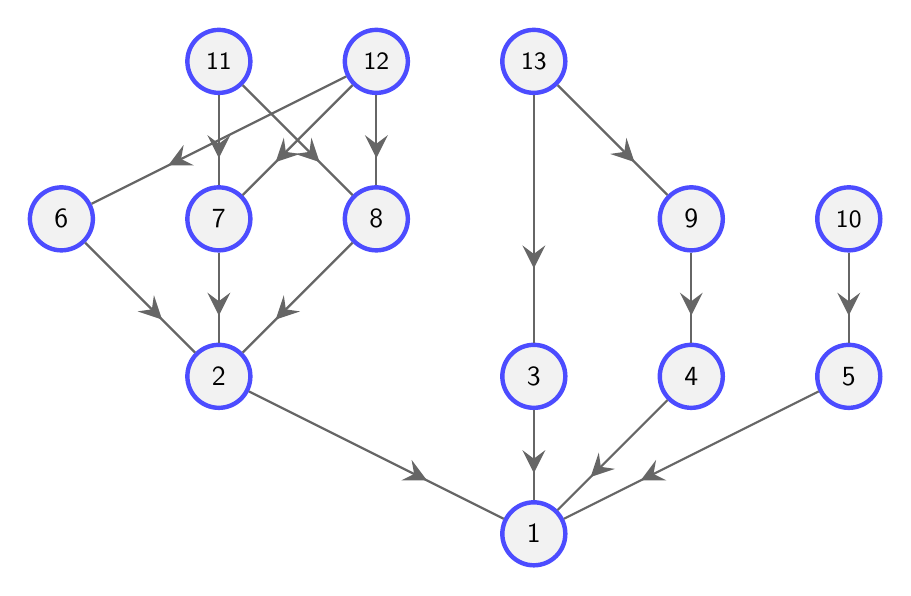
\begin{tikzpicture}[font=\sffamily]
% nodes
\begin{scope}[every node/.style={circle,draw=blue!70, fill=gray!10, ultra thick, minimum size=8mm}]
	\node(A) at (6,0) {1};
	\node(B) at (2,2) {2};
    \node(H) at (6,2) {3};
    \node(I) at (8,2) {4};
    \node(J) at (10,2) {5};
    
    \node(C) at (0,4) {6};
    
    \node(D) at (2,4) {7};
    \node(E) at (4,4) {8};
    \node(F) at (2,6) {\small 11};
    \node(G) at (4,6) {\small 12};

    \node(K) at (8,4) {9};
    \node(L) at (10,4) {\small 10};
    \node(M) at (6,6) {\small 13};
\end{scope}
\begin{scope}[thick, draw=black!60, decoration={
    markings,
    mark=at position 0.7 with {\arrow[scale=2,>=stealth]{>}}}
    ] 
\draw[postaction={decorate}] (B) -- (A);   
\draw[postaction={decorate}] (C) -- (B); 
\draw[postaction={decorate}] (D) -- (B); 
\draw[postaction={decorate}] (E) -- (B); 
\draw[postaction={decorate}] (F) -- (D); 
\draw[postaction={decorate}] (F) -- (E); 
\draw[postaction={decorate}] (G) -- (E); 
\draw[postaction={decorate}] (G) -- (D); 
\draw[postaction={decorate}] (G) -- (C); 
\draw[postaction={decorate}] (H) -- (A); 
\draw[postaction={decorate}] (I) -- (A); 
\draw[postaction={decorate}] (J) -- (A); 
\draw[postaction={decorate}] (K) -- (I); 
\draw[postaction={decorate}] (L) -- (J); 
\draw[postaction={decorate}] (M) -- (K); 
\draw[postaction={decorate}] (M) -- (H); 
\end{scope}
\end{tikzpicture}
\caption{labeling phase in the Coffman-Graham algorithm}
\label{fig:C-G_labeling}
\end{figure}


Scheduling phase of the Coffman-Graham algorithm is illustrated as follows~\cite{leung_basic_2004,coffman_optimal_1972}:
Whenever a processor is free for assignment, assign that ready task with the highest label among all ready jobs to it. 

Let $W$ be the number of processors, $\omega$ be the length of a schedule produced by the algorithm, and $\omega_0$ be the length of an optimal schedule, then $\omega/ \omega_0 \leq 2-2/W$~\cite{coffman_optimal_1972,lam_worst_1977}. 


\subsection{Hu's Algorithm}
Given a fixed width $w$, Hu's algorithm can find a schedule for a finite number of tasks which all require unit time to complete in $O(|V|\log |V|)$ time~\cite{leung_basic_2004}. Hu's algorithm minimizes the total completion time for a set of tasks restricted by precedence tree constraints, and is optimal~\cite{mchugh_hus_1984}.

Similar to the Coffman-Graham algorithm, Hu's algorithm also has labeling and scheduling phases. However, they are differentiated by they way of labeling. In Hu's algorithm, the label of a task is a function of the \textit{level} of the task~\cite{huo_online_2005}. Let a final task be a task without any successors. Final tasks all receive a label $1$ at the beginning of the labelling process. Assume each task require 1 unit of time to finish, then a task $v$ is labelled with $\alpha(v)=x_v + 1$, in which $x_v$ is the length of the longest path from $v$ to the final task in graph~\cite{hu_parallel_1961}. Figure~\ref{fig:huAlg} by Hu gives an example of labeling process in a graph. For a node $v$ in the figure, the number that appears in $v$ is $v$'s label $\alpha(v)$.

The scheduling phase is similar in Hu's algorithm as in the Coffman-Graham algorithm despite the fact that tasks can have the same label in Hu's algorithm. Assume that we will schedule for $W$ processors, and each processor can only execute one task at a time. Whenever a processor is free for assignment, assign the task with the largest label among all ready tasks to the processor. Repeat until all tasks are assigned. When some ready tasks have the same label, break the tie arbitrarily~\cite{leung_basic_2004}. In other words, it selects a ready task that has the longest distance to a final task. We then assign it to the highest layer we currently have. If the number of tasks in this layer is equal to the layer width $W$, it creates a new layer above this layer and assign the task to the new layer. 

\begin{figure}[ht]
\centering
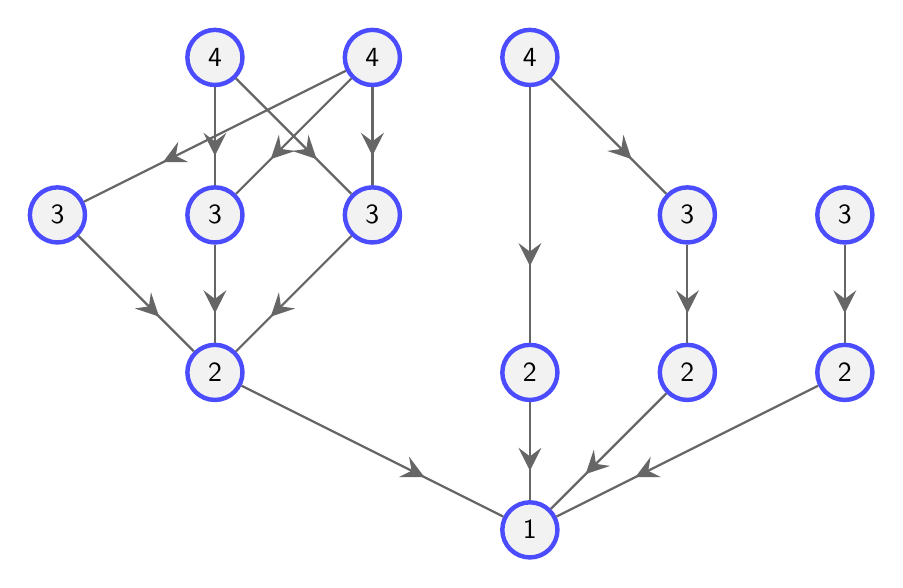
\begin{tikzpicture}[font=\sffamily]
% nodes
\begin{scope}[every node/.style={circle,draw=blue!70, fill=gray!10, ultra thick, minimum size=7mm}]
	\node(A) at (6,0) {1};
	\node(B) at (2,2) {2};
    \node(C) at (0,4) {3};
    \node(D) at (2,4) {3};
    \node(E) at (4,4) {3};
    \node(F) at (2,6) {4};
    \node(G) at (4,6) {4};
    \node(H) at (6,2) {2};
    \node(I) at (8,2) {2};
    \node(J) at (10,2) {2};
    \node(K) at (8,4) {3};
    \node(L) at (10,4) {3};
    \node(M) at (6,6) {4};
\end{scope}
\begin{scope}[thick, draw=black!60, decoration={
    markings,
    mark=at position 0.7 with {\arrow[scale=2,>=stealth]{>}}}
    ] 
\draw[postaction={decorate}] (B) -- (A);   
\draw[postaction={decorate}] (C) -- (B); 
\draw[postaction={decorate}] (D) -- (B); 
\draw[postaction={decorate}] (E) -- (B); 
\draw[postaction={decorate}] (F) -- (D); 
\draw[postaction={decorate}] (F) -- (E); 
\draw[postaction={decorate}] (G) -- (E); 
\draw[postaction={decorate}] (G) -- (D); 
\draw[postaction={decorate}] (G) -- (C); 
\draw[postaction={decorate}] (H) -- (A); 
\draw[postaction={decorate}] (I) -- (A); 
\draw[postaction={decorate}] (J) -- (A); 
\draw[postaction={decorate}] (K) -- (I); 
\draw[postaction={decorate}] (L) -- (J); 
\draw[postaction={decorate}] (M) -- (K); 
\draw[postaction={decorate}] (M) -- (H); 
\end{scope}
\end{tikzpicture}
\caption{labeling process in Hu's algorithm~\cite{hu_parallel_1961}}
\label{fig:huAlg}
\end{figure}
\section{Proposed Method}
\subsection{Problem Formulation and Term Definition}
\subsubsection{Schedule}
A schedule $L$ is represented as a list of layers. Each layer stands for a quarter in the actual schedule, and it holds a set of assigned courses. The first layer $L_0$ in the schedule is the bottom layer.

\subsubsection{Width Bound}
$W$ is a table of width bound for different layers in schedule. The maximum width of layer $L_i$ is $W(L_i)$, which is the maximum total units of courses in it. We can also define a key called $others$ in $W$ such that if there is no specified width bound for a layer in $L$, its width bound is $W(others)$.

$M$ is a table storing current current total number of units in each layer during the assignment process. Every time when a course $v$ is assigned to a layer $L_i$, we update $M(L_i)=M(L_i)+v.Units$.
\subsubsection{Upper Bound}
Because during the assignment, we may assign a course to a new layer even if the width of current top layer does not reach the maximum,
we are not able to estimate the upper bound at the beginning. We specify an upper bound layer index $u$ for layers instead. 
\subsubsection{Requirements table}
Requirements $R$ contains a table of requirements. A requirement is in the following format:
    \begin{displayquote}
    $n$ courses in:\\
    (Course1, Course2, Course3)\\
    \textbf{AND}\\
    $m$ courses in:\\
    (Course4, Course5, Course6)
    \end{displayquote}
$n$ and $m$ is the number of courses required in the set of courses. Both the number of sets and the number of the courses in the set are not fixed.
Let the name of a requirement be $k$, the index of the a set \textit{(Course1, Course2, Course3)} be $i$, and the number of courses required for this set be $n$. Then we get $R_k^i=n$. 




\subsubsection{Course}
Each course in our course scheduling problem represents a vertex in graph. A course $v$ contains the following information:
\begin{itemize}
    \item $v.Units$: Total units $v$ requires. If $v$ has a $4$ units lecture section, and a $1$ unit lab section, it requires $5$ units in total.
    \item $v.QuarterCodes$: In what quarters the department offers this course. There is a presumption in both the Coffman-Graham algorithm and Hu's algorithm that all tasks are available at any time in the schedule. However, a course may not be offered in every quarter and every year, which means that not every layer can hold this course. Therefore, knowing when a course will be offered is significant in the scheduling phase.
    
    We stores quarter information for the latest $2$ years, $6$ quarters in total for testing. The latest year is called \textit{odd year}, the the second latest year is \textit{even year}. Each quarter has a quarter code, and if a course is offered in a quarter, we add this quarter code in quarters information. If year 2017 is the latest year, we have:
    \begin{center}
    \begin{tabular}{ |l|c| } 
         \hline
         quarter name & quarter code \\
         \hline
         2017 Fall & 0 \\ 
         2017 Winter & 1 \\ 
         2017 Spring & 2 \\ 
         2016 Fall & 3 \\
         2016 Winter & 4 \\
         2016 Spring & 5 \\
         \hline
    \end{tabular}
    \end{center}
    Using quarter codes can help matching layer indices with a corresponding quarter using a mod operation. For example, with 0-indexing, if a layer has index equal to $8$, then we calculate $8 \bmod 6 = 2$, so the quarter code for this layer is $2$. 
    \item $v.IsUpperOnly$: It denotes if $v$ is an upper only course. If it returns $true$, it means $v$ is an upper standing only course. Suppose there is an integer $U$ representing upper units and $U \geq 0$, then an upper standing course requires a student to achieve at least $U$ units before they can take it. 
    
    Thus, if $v.IsUpperOnly=true$, $v$ can only be assigned to a layer $L_i$ such that \[(\sum_{k=0}^{i-1} \sum u.Units, \forall u\in L_k) \geq U\]
    
    \item $v.Prerequisite$: The prerequisite of $v$ has the following input format:
    \begin{displayquote}
    Course1\\
    \textbf{AND}\\
    (Course2 \textbf{OR} Course3)\\
    \textbf{AND}\\
    (Course4 \textbf{OR} Course5 \textbf{OR} Course6)
    \end{displayquote}
    This format is in the conjunctive normal form (CNF), which is an AND of ORs, and can be represented as:
    $$((Course1) \wedge (Course2 \vee Course3) \wedge (Course4 \vee Course5 \vee Course6) $$
    It is noted that the number of courses in each OR is not fixed.
    Based on this structure, we have two sequences $A_v$ and $B_v$ for a single course $v$. $A_v$ represents an AND sequence, which holds a list of OR sets. Each OR set consists of a set of prerequisite courses for $v$. The OR set with index $i$ in $v$'s AND sequence is $A_v^i$. A prerequisite course $u$ is in $A_v$ if it is in one of the OR set of $A_v$.
    
    $B_v$ in $B$ stores information about how $v$ is satisfied. In $B_v$, $B_v^i$ refers to the OR set $A_v^i$ in $A_v$. Initially, $B_v^i$ is null. If a course $u$ is assigned to the schedule, $u$ is in $A_v^i$, and $B_v^i$ is null, we set $B_v^i=u$, showing that OR set $A_v^i$ is satisfied by $u$. If and only if all OR sets in $A_v$ are satisfied, then the AND sequence $A_v$ is fully satisfied, and the course's prerequisite is also fully satisfied. We call this a ready course because it is ready to be assigned to the schedule. 
    \item $v.Successors$: A set of courses. For each course $w$ in $v.Successors$, there exists $A_w^i \in A_w$ such that $v \in A_w^i$.  
    \item $v.Requirements$: A set of requirements that $v$ can satisfy.
    Each element in the set is represented as a tuple $(k,i)$ for $k$ is a requirement name and $i$ is the index of a set in $R_k$ such that $v\in R_k^i$. 
    Having this information in $v$ can help finding its satisfying requirements in the requirement table in linear time time after $v$ is assigned. 
    \item $v.CourseValue$: The number of requirements $v$ meets, that is the length of $v.Requirements$. 
    \item $v.DependentIndex$: The largest layer index of $v$'s dependent schedule. Initially, $v.DependentIndex=0$.
\end{itemize}
% Information above is necessary for generating a schedule.
\subsubsection{Graph}
A graph for course scheduling is a collection of courses. A course $v$ has incoming edges from each course $u\in A_v$. Similarly, $v$ has outgoing edges to each course $w\in v.Successors$. Note that edges can also be reversed to the find longest path distance required in ~\ref{HuAlgorithm}. 

We define graph to be $G=(V,E)$, a graph $G$ with $|V|$ courses and $|E|$ edges. $G$ is a directed acyclic graph. Suppose there is a cycle in $G$, and course $v$ is in the cycle, then $v$'s successor will become its prerequisite, and we can never assign $v$ to the schedule. Although it is not required to do transitive reduction on $G$, doing so can decrease $|E|$ of $G$. 

\subsection{Single Course Assignment}
\textcolor{red}{This part needs modification later because I find another possible way to find the smallest valid layer using math in linear time -- need further discussion}

For a course $v$, we define a layer $L_i$ with $M(L_i) + v.Units < W(L_i)$ and $(i \bmod 6)\in v.QuarterCodes$ to be a valid layer of $v$. To simplify, we define two functions $Valid$ and $HasDependent$. $Valid(L_i,v)$ returns true if $L_i$ is a valid layer for $v$. $HasDependent(L_i,v)$ returns true if $i<v.DependentIndex$.

In course scheduling algorithm, after a ready course $v$ is selected, if the highest layer is valid, it marks this layer to be a lowest valid layer. Otherwise, it creates new layers above the highest layer until the new layer is valid, and marks this new layer as the lowest valid layer. Then it starts to scan the schedule from the original second highest layer and renew the lowest valid layer. Whenever it finds a layer that contains any courses in $v.Prerequisite$ or it reaches the upper bound layer, it stops scanning and assigns $v$ to the lowest valid layer.

Algorithm~\ref{alg:AssignCourse} below shows the scheduling process for a single course $v$. 
% The schedule has at least one empty layer at the beginning of the process.

\begin{algorithm}[H]
\DontPrintSemicolon
\SetKwInOut{Input}{Input}
\SetKwInOut{Output}{Output}

\Input{graph $G=(V,E)$, course $v$, Schedule $L$, upperBound index $u$}
\Output{the index of the layer where $v$ is assigned}
step = $|L|-1$\;
\uIf{$Valid(L_{step}, v)= false$ \textbf{or} $HasDependent(L_{step}, v)= true$
}{
    \Do{$Valid(L_i,v) = false$ \textbf{and} ($v.IsUpperOnly=false$ \textbf{or} $i<u$)}
    {add new empty layer $L_i$ above current highest layer}
    }
lastStep = $|L| -1$ \;
\While{$v$ is not assigned \textbf{and} ($v.IsUpperOnly=false$ \textbf{or} $step\geq u$)}{
\uIf{$HasDependent(L_{step},v)=true$}{
    add $v$ to $L_{lastStep}$\;
    return\;
    }
\uElseIf{$Valid(L_{lastStep}, v) = true$}{
    lastStep = step}
    step = step -1\;
}
\uIf{$v$ is not assigned}{
    assign $v$ to layer $L_{lastStep}$
    }
    return lastStep\;

\caption{AssignCourse}\label{alg:AssignCourse}
\end{algorithm}
\bigskip
In algorithm~\ref{alg:AssignCourse}, $step$ represents the current scanning layer index. With 0-indexing, $|L|-1$ is the highest layer index in schedule $L$. $lastStep$ represents the current lowest valid layer for course $v$. 

To assign a single course, the algorithm checks at most $|L|$ layers in the schedule. Suppose each layer holds at least one course, then in the worst case, there is only one course for each layer, so$|L|\leq |V|$. The time complexity for  algorithm~\ref{alg:AssignCourse} is $O(|L|)=O(|V|)$. 


\subsection{Implementation of Hu's Algorithm}\label{HuAlgorithm}

Unlike the precedence-constrained mulitprocessor scheduling problem, in which each task is ready if all of its immediate predecessors are assigned into the schedule, our algorithm does not require all courses in the prerequisite to be scheduled. 

Although the relationship between each course is not a strict precedence-constrained relationship, inspired by Hu's algorithm, we can reverse the graph, and find the longest path from a course to another course that does not have any successors. 

In order to reverse the graph $G$, we define for each prerequisite course $u \in A_v$, we have an edge $(v,u)$ from $v$ to $u$, instead of from $u$ to $v$.
Because we prefer to assign those courses that can meet more requirements first, we also use a heuristic function for labeling. Label of $v$, $\alpha(u) = \alpha(v)+u.CourseValue$. If $v$ does not have any successors, $\alpha(v)=v.CourseValue$. Because we view $v.CourseValue$ as the weight of edge $(v,u)$, we can use DAG shortest path algorithm with modifications to generate a topological ordering and find the longest path from a course to another course without any successors. When we are looping through all courses in $G$, we can also remove any courses that do not satisfy any requirements.
Algorithm~\ref{alg:labeling} bellow illustrates this procedure. 

\begin{algorithm}[H]
\Input{graph $G$}
\Output{labeled graph $G$}
\For{each course $v \in G$}{
    \uIf{$v.courseValue = 0$}{
        $G.remove(v)$}
    \uElseIf{$v.successors \neq \emptyset$ }{
        $\alpha(v) = -\infty$}
    \Else{$\alpha(v)= c.courseValue$}
    }
\For{each course $v\in G$ in topological ordering}{
        \For{each $u \in A_v$}{
        $\alpha(u) = max((\alpha(u)+v.courseValue), \alpha(u))$
        }
    }
return $G$

\caption{Labeling}\label{alg:labeling}

\end{algorithm}
\bigskip
In algorithm~\ref{alg:labeling}, the first for loop takes $O(|V|)$ time to initialize labels for all vertices in $G$, and the second for loop takes $O(|V|+|E|)$ time to visit all vertices and edges in $G$ and correct label of each course. The total time required is $O(|V|+|E|)$.

\subsection{Course Scheduling Algorithm}
Due to the limitation of finding an upper bound without getting an actual schedule, we have to first input a range of upper bounds to the algorithm, and then generate $m-n+1$ schedules. After that, we check the validity of schedules and pick the best schedule that has the minimum number of layers among all valid schedules it generates. Algorithms required for scheduling are presented below: 

\begin{algorithm}[H]
\Input{graph $G$, upper bounds range $[m,n]$, initial units $initUnit$, upper standing units $upperUnit$}
\Output{best schedule $bestL$}
Labeling($G$)\;
bestL = Null\;
\For{$u\gets m$ to $n$}{
    L = CourseScheduling($G,u$)\;
    totalUnit = $initUnit$\;
    \uIf{$|L|<|bestL|$}{
    \For{each layer $L_i\in L$}{
        layerUnit = 0\;
        \For{each course $v\in L_i$}{
            \uIf{$v$ is upper only \textbf{and} totalUnit$<$upperUnit }{
            reject schedule $L$}
            layerUnit = layerUnit + $v$.units
        }
        totalUnit = totalUnit + layerUnit
    }
    
    \uIf{$L$ is not rejected}{
        $L = bestL$}
        }
}
return bestL\;

\caption{CourseScheduling}\label{alg:coursescheduling}
\end{algorithm}
\bigskip
\begin{algorithm}[H]
\Input{graph $G$, upper bound index $u$}
\Output{Schedule $L$}
Create priority queue $Q$ using course label as key\;
Create schedule with an empty layer $L$\;
\For{each $course v \in G$}{
    \uIf{$v.successors = \emptyset$}{
        Q.enqueue((v, v.label))\;}  
}
\While{$Q$ is not empty}{\label{alg:getSchedule:while}
    current = Q.extractMax()\;
    \uIf{current satisfies any requirements}{
    assingnedIndex = AssignCourse($G, current, L, u$)\;
    ExpandQueue($current, Q, assingnedIndex$)\;
    }
    \tcp{update requirement table with $current$}
    \For{each $(k,i)\in v.Requirements$}{
        \uIf{$R_k^i > 0$}{
            $R_k^i= R_k^i-1$}
        }
}
return $L$\;
\caption{GetSchedule}\label{alg:getSchedule}
\end{algorithm}
\bigskip
\begin{algorithm}[H]
\Input{course $v$, priority queue $Q$, assignedIndex $index$}
\For{each course $u \in v.successors$}{
    allNotNull=true\;
    \For{$i\gets 0$ to $|A_u|-1$}{
        \uIf{ $B_u^i=Null$}{
        \uIf{$v \in A_u^i$}{
        $B_u^i = v$\;
        $u.DependentIndex = max(u.DependentIndex, index) $
        }
        \Else{allNotNull = false\;}
        }
    }
    \uIf{$allNotNull=true$}{
    Q.enqueue((u, $\alpha(u)$))}
}
\caption{ExpandQueue}\label{alg:ExpandQueue}
\end{algorithm}



\bigskip

Algorithm~\ref{alg:getSchedule} presents how it generates a schedule with a specific upper bound $u$. After the course is assigned, algorithm~\ref{alg:ExpandQueue} visits each edge going out from the course $current$ to another course $u$ and updates $B_u$. If $u$ is ready, it inserts $u$ to the priority queue. The priority queue $Q$ is implemented with a max-heap structure with course label as the key. Since each enqueue or dequeue operation takes $O(\log |V|)$ time and runs $O(|V|)$ times, the total time required on $Q$ is $O(|V|\log|V|)$. In the while loop, each time AssignCourse~\ref{alg:AssignCourse} takes $O(|V|)$ time to assign a course, and ExpandQueue~\ref{alg:ExpandQueue} visits all outgoing edges of the course. Therefore, it takes $(O(|V|^2+|E|)+O(|V|\log|V|)=O(|V|^2)$ time to get a schedule. 

Algorithm~\ref{alg:coursescheduling} shows how it gets the best schedule within a range of upper bounds from layer index $m$ to $n$. The labeling phase in it takes $O(|V|+|E|)$ time. Time required for algorithm~\ref{alg:getSchedule} still dominates, so the total time is $O(|V|^2)$.

\section{Experimental Result}

In the research, we implement the course scheduling algorithm using Python~\footnote{\url{https://github.com/jennyzeng/CourseScheduling}}. We test the quality of our algorithm by simulating a course schedule for a student majoring in Computer Science and specializing in Intelligent Systems. Some other specifications are:
\begin{enumerate}
    \item Besides major requirement, the student is also required to satisfy General Requirements;
    \item The student can only take at most 12 units at the first quarter and at most 18 units for the rest of the quarter;
    \item The student has 0 default units at the beginning of assignment;
    \item Upper bound range $U$ is from 0 to 10, inclusive;
    \item First quarter of schedule is 2016 fall quarter. 
\end{enumerate}
With data collected on UCI website~\footnote{\url{http://catalogue.uci.edu/} and \url{https://www.reg.uci.edu/perl/WebSoc}}, we get the following result:

\begin{center}
\begin{tabular}{|m{1cm}|m{2cm}|m{2cm}|m{2cm}|m{2cm}|m{2cm}|}
\hline
\textbf{Code} & \multicolumn{5}{c|}{\textbf{Courses}}                                                  \\ \hline
0            & ICS 31  & MATH 2A        & ICS 6B      &                 &            \\ \hline
1            & ICS 32  & MATH 2B        & ICS 51+51L      & ICS 6D      &            \\ \hline
2            & ICS 33  & STATS 67       & MATH 3A         & WRTNG-LOW 1 &            \\ \hline
3            & ICS 45C & CS 151    & CS 169     & HIST 40A     & ICS 90 \\ \hline
4            & ICS 46  & CS 121    & CS 178     & HIST 40B     &            \\ \hline
5            & HIST 40C & POLSCI 21A     & GEII-1          & GEIII-1         &            \\ \hline
6            & CS 161 & CS 171    & GEIII-2         & GEVI-1          &            \\ \hline
7            & CS 116 & CS 125    & CS 162     & CS 175     &            \\ \hline
8            & CS 163 & CS 177    & GEVII-1         & GEVIII-1        &            \\ \hline
9            & CS 113 & IN4MATX 43     & WRTNG-LOW 2 &                 &            \\ \hline
10           & CS 164 & ICS 53+53L & ICS 139W    &                 &            \\ \hline
\end{tabular}
% \end{table}
\end{center}
In table above, the Code column shows layer index. Code $0$ stands for the first layer (quarter). Course columns present the courses assigned to a layer. The algorithm generates a schedule with 10 layers, equivalent to 3 years and 2 quarters. It prefers to assign major courses rather than general requirement courses first because they have a larger label value: they only satisfy one requirement, and they do not have any successors. Moreover, it states layer 5, the spring quarter of the second year, is the best upper bound for scheduling because we can get a schedule with the smallest number of layers among all valid schedules. 

\section{Conclusion and Future work}
Through examining two task scheduling algorithms, the Coffman-Graham algorithm and Hu's algorithm, we are able to develop our own scheduling algorithm that works for course scheduling in time $O(|V|^2)$. Looking at the experimental result, the schedule we generate for a student is reasonable and valid based on the provided constraints. With this algorithm, programmers can develop an application to assist students and counselors to make a study plan. 

However, it is noted that building such a schedule is still time consuming, and applying better data structures can possibly reduce the total running time. Furthermore, after adding many constraints for the algorithm, we can only test the quality of the schedule based on the experimental results. Although the result is workable for a Computer Science student, because we are not able to access the database for courses and student requirements at UCI, we cannot evaluate the quality of schedule generated by the algorithm thoroughly.


\newpage
\bibliographystyle{ieeetr}
\bibliography{ref}
\end{document}
